\section{Auswertung}
\label{sec:Auswertung}

\subsection{Filterkurve des Selektiv-Verstärkers}

In diesem Versuchsteil soll die Filterkurve des verwendeten Selektiv-Verstärkers bei 
einer Güte von $Q=20$ untersucht werden.\\
Es werden bei immer höheren Frequenzen des Sinusgenerators eingestellt und die resultierenden
Spannungen im Wechselstrom-Milli-Voltmeters abgelesen. Die aufgenommenen Werte sind in 
\autoref{tab:Filterkurve} zu sehen. Es wurde eine Verstärkung von x10 verwendet. Die eigentlich
resultierenden Spannung sind also nur 0,1x so groß wie die in der Tabelle angegebenen.\\

\begin{table}
  \centering
  \caption{Gemessene Ausgangsspannungen in Abhängigkeit der Frequenz des Sinusgenerators.}
  \label{tab:Filterkurve}
  \begin{tabular}{c | c || c | c}
    \toprule
    Frequenz $f$ / kHz & Ausgangsspannung $U_{\mathrm{A}}$ / V & Frequenz $f$ / kHz & Ausgangsspannung $U_{\mathrm{A}}$ / V \\
    \hline
    10,17 &  0,16  &  22,10 &  8,50 \\
    13,81 &  0,36  &  22,40 &  7,00 \\
    18,23 &  0,90  &  23,10 &  2,90 \\
    19,40 &  1,50  &  24,40 &  1,00 \\
    20,10 &  2,40  &  26,10 &  0,50 \\
    21,00 &  5,20  &  30,80 &  0,30 \\
    21,50 &  8,30  & & \\
    \midrule
    \bottomrule
  \end{tabular}
\end{table}

Die aufgenommenen Messwertpaare werden nun in einem Diagramm gegeneinander geplotted. Die 
enstehende Graphik zeigt wie zu erwarten eine Glockenkurve nach der Gleichung
\begin{equation*}
  U(f) = e^{-a(f-\nu_0)^2}.
\end{equation*}
Die Graphik mitsamt der mit Python gefiteten Glockenkurve ist in ... zu sehen.\\
Damit die Graphik besser zu lesen ist, werden die Messwerte der Spannung relativ zur 
maximal gemessenen Spannung $U_{\mathrm{max}} = 8,5 \si{\volt}$ geplotted. Der in der Formel
der Glockenkurve verwendeten Parameter $\nu_0$ gibt die Verschiebung der Glockenkurve an.
Mittels der Python library scipy wurde ein Wert von $\nu_0 = (21,79 \pm 0,07) \, \si{\kilo\hertz} $
berechnet. Für den Parameter $a$ gibt Python den Wert 
$a = (0,52 \pm 0,07 ) \, \si{\per\square\kilo\hertz}$.\\
\begin{figure}
  \centering
  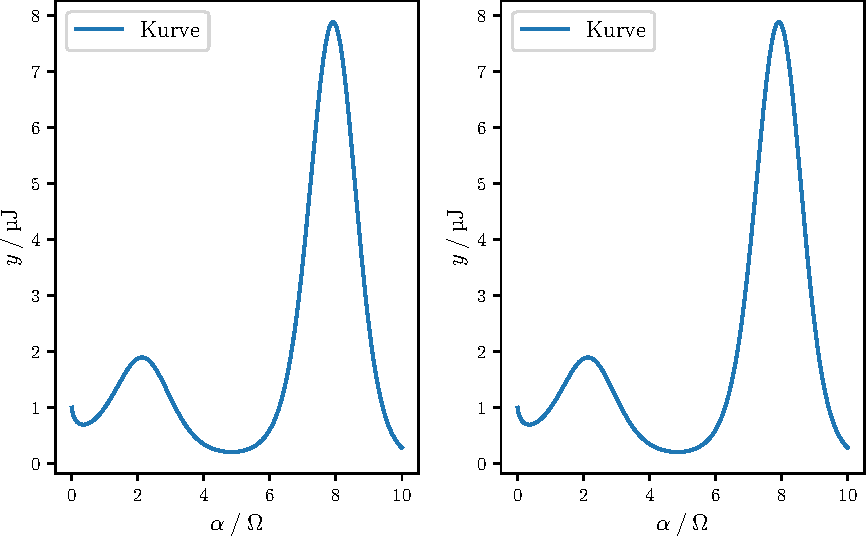
\includegraphics[width=1\textwidth]{build/plot.pdf}
  \caption{Filterkurve des Selektiv-Verstärkers.}
  \label{Abb:Absorption}
\end{figure}
Die Frequenzen $\nu_{-}$ und $\nu_{+}$ sind die Schnittpunkte des Fits mit der Geraden
$f(x) = \frac{1}{\sqrt{2}}$. Die Schnittstellen wurden mittels eines Grafischen Taschenrechners
ermittelt und ergaben die Werte $\nu_{-} = 20,97 \, \si{\kilo\hertz}$ und $\nu_{+} = 22,60 \, \si{\kilo\hertz}$.\\
Mit ... lässt sich nun die Güte bestimmen. Mit Gaußscher Fehlerfortpflanzung ergibt sich
für die zu untersuchende Filterkurve $Q = (13,37 \pm 0,04)$.\\
Die relative Abweichung zu unserem Theoriewert $Q^* = 20$ lässt sich mit der Gleichung
\begin{equation*}
    \Delta_{\mathrm{rel}}(Q) = \frac{|Q^* - Q|}{Q^*}
\end{equation*}
berechnen. Einsetzen ergibt den Wert $\Delta Q = 33,15 \%$.\\

\subsection{Bestimmung der Suszeptibilitäten drei seltener Erden}

Siehe \autoref{fig:plot}!
